\documentclass[10pt]{beamer}

  % Math Packages
  \usepackage{amsmath}
  \usepackage{amsthm}
  \usepackage{mathtools}

  % Graphics Packages
  \usepackage{graphicx}
  \graphicspath{ {../_static/images/} }
  \usepackage{pgf}
  \usepackage[export]{adjustbox}

  % Code listings
  \usepackage{listings}
  \lstset{language=Python, basicstyle=\scriptsize, showstringspaces=false}

  % Misc packages
  \usepackage{hyperref}
  \hypersetup{colorlinks=true,linkcolor=,urlcolor=blue}

  % Colors
  \definecolor{myblue}{RGB}{25,98,148}
  \definecolor{mygray}{RGB}{66,66,66}

  % Theme Settings
  \usetheme[subsectionpage=progressbar]{metropolis}

  % \setbeamercolor{normal text}{fg=mygray}
  % \setbeamercolor{alerted text}{fg=myblue}
  % \setbeamercolor{title text}{fg=mygray}
  % \setbeamercolor{title separator}{fg=myblue}
  % \setbeamercolor{progress bar}{fg=myblue}
  % \setbeamercolor{frametitle}{bg=myblue}


\title{Package testing}

\date[]{\today}

\begin{document}

% Title Slide
\begin{frame}
  \titlepage
\end{frame}


% ------------------------------ %
% Unit and integration testing
% ------------------------------ %
\section{Unit, integration, and system testing}

  \begin{frame} \frametitle{Types of testing: analogy}

    We will describe the different types of testing using the analogy of building a car.

    \vspace{0.25cm}

    Consider a car that consists of four components:

    \begin{enumerate}
      \item An engine
      \item An axle
      \item An interior
      \item A frame
      \item Four wheels
    \end{enumerate}

  \end{frame}

  \begin{frame} \frametitle{Types of testing: unit testing}

    Unit testing involves testing a single component at a time to make sure that it
    behaves as you expect in isolation.

    \vspace{0.25cm}

    For example, in our car analogy, we might check whether the engine ran and whether
    pistons operated at correct frequency, etc\dots

    \vspace{0.25cm}

    \textbf{What are other examples of unit testing in the context of our car?}

  \end{frame}

  \begin{frame} \frametitle{Types of testing: integration testing}

    Integration testing is aimed at ensuring each part works well with the parts that
    it is intended to interace with.

    \vspace{0.25cm}

    For example, in our car analogy, we might check whether the engine was successfully
    able to turn the wheels through its connection on the axle.

    \vspace{0.25cm}

    \textbf{What are other examples of integration testing in the context of our car?}

  \end{frame}

  \begin{frame} \frametitle{Types of testing: system testing}

    System testing is aimed at ensuring all parts work well with one another in an
    environment similar to one that the software might be operated in

    \vspace{0.25cm}

    For example, in our car analogy, this might involve taking some of the cars that
    are produced for a drive in the parking lot

    \vspace{0.25cm}

    \textbf{What are other examples of system testing in the context of our car?}

  \end{frame}


% ------------------------------ %
% Testing and project management
% ------------------------------ %
\section{Testing and project management}

  \subsection{Test-driven development}

  \begin{frame} \frametitle{Test-driven development}

    Test-driven development is focused on the repitition of a very short development cycle

    It begins with the idea of a particular requirement or feature and then developing
    with tests at the center of the (short!) development cycle

  \end{frame}

  \begin{frame} \frametitle{Test-driven development: Steps}

    {\small
    Once there is a new requirement or feature that you'd like to add, the development
    cycle follows these steps\footnote{The
    \href{https://en.wikipedia.org/wiki/Test-driven_development}{Wikipedia article} on
    test-driven development is excellent!}:

    \begin{enumerate}
      \item Add tests: You can consider your feature ``implemented'' once it can pass
        this set of tests
      \item Run the test suite: Make sure your new tests don't already pass before you've
        implemented the new functionality
      \item Add the new feature: Only do what is necessary here to pass the \textit{new}
        test
      \item Run the test suite: Ensure that the code you've added passes the new test and
        that it doesn't cause any of the previous tests to break
      \item Refactor code: Since the development in step 3 is only about getting the test
        to pass, you will need to think about how it fits into your software design at
        this stage. You may find it necessary to modify both the recently added code AND
        the previously written code
    \end{enumerate}
    }

  \end{frame}

  \begin{frame} \frametitle{Test-driven development: steps}

    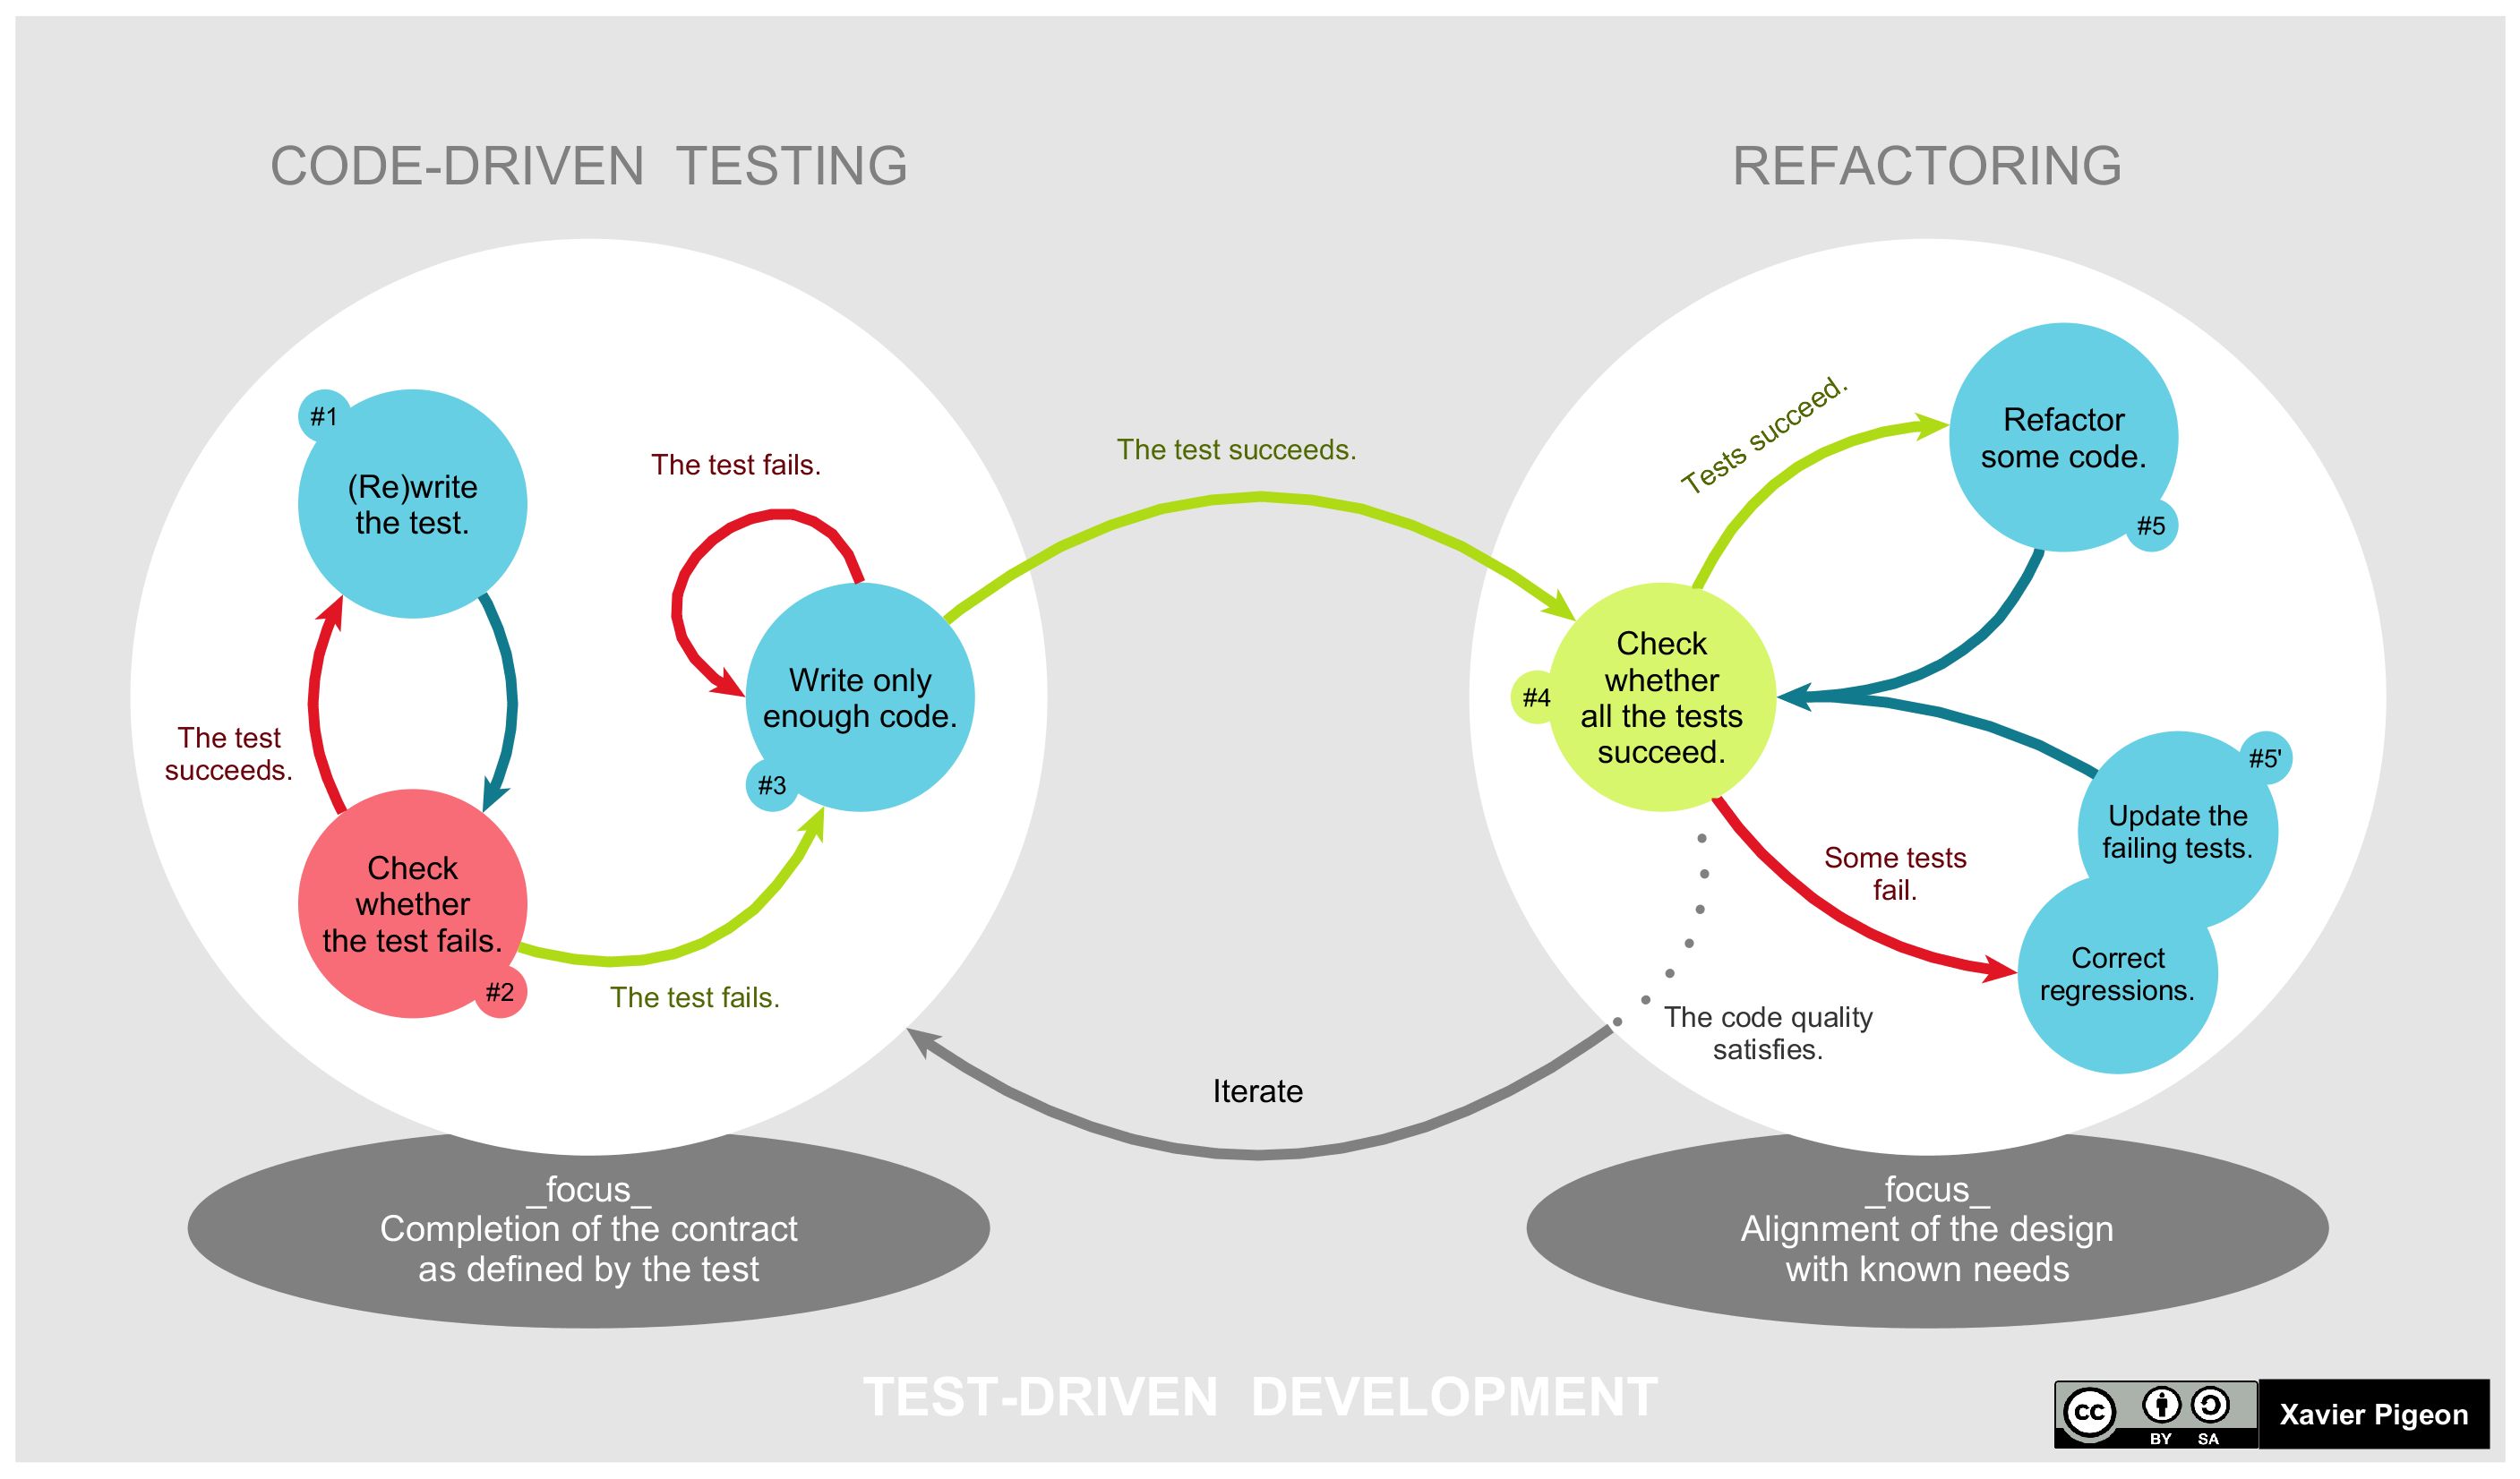
\includegraphics[width=0.9\textwidth]{TDD_Global_Lifecycle}

    \tiny{Figure attribution: By Xarawn - Own work, CC BY-SA 4.0, https://commons.wikimedia.org/w/index.php?curid=44782343}

  \end{frame}


% ------------------------------ %
% Writing tests
% ------------------------------ %
\section{Testing in Python}

  \begin{frame} \frametitle{Two main testing frameworks}

    \texttt{unittest} is a testing library that's built into the Python standard library.
    This means that you will always have access to this library if you're running Python.

    \vspace{0.25cm}

    \texttt{pytest} is a flexible and powerful testing framework. Many neat features
    that are worth exploring if you end up writing a relatively large test set.

  \end{frame}

  \begin{frame} \frametitle{unittest}

    We are going to focus on \texttt{unittest} today because everyone should have it
    installed already and it should cover our use cases for today

  \end{frame}

  \begin{frame} \frametitle{unittest: \texttt{unittest.TestCase}}

    The base component of \texttt{unittest} is the \texttt{unittest.TestCase} class

    \vspace{0.25cm}

    All tests are created by subclassing this class

  \end{frame}

  \begin{frame}[fragile] \frametitle{unittest: \texttt{unittest.TestCase}}

      \begin{lstlisting}{TestCase}
      import unittest

      class TestRandomStuff(unittest.TestCase):

          def test_addition(self):
              self.assertEqual(1 + 1, 2)

          def test_upper(self):
              self.assert('foo'.upper(), 'FOO')

      if __name__ == '__main__':
          unittest.main()

      \end{lstlisting}

      Can run this with \texttt{python -m unittest} (can add \texttt{-v} at end if
      you would like verbose output)

  \end{frame}

  \begin{frame} \frametitle{Using unittest}

    \textbf{Step 1}: Create a folder for all of your tests --- I like to use
    \texttt{<package>/test} but others argue for putting it closer to the source code
    in \texttt{<package>/<package>/test}

    \vspace{0.25cm}

    \textbf{Step 2}: Write test classes in files that begin with the word \texttt{test}
    --- You can use a different pattern, but you have to specify it when you run the
    tests

    \vspace{0.25cm}

    \textbf{Step 3}: Run tests

  \end{frame}

  \begin{frame} \frametitle{\texttt{unittest.TestCase} features: setup and teardown}

    The \texttt{setUp} and \texttt{tearDown} are meant to support examples in which you
    require some form of temporary feature, for example, if you needed a database to run
    a test, then you could create a fresh database in \texttt{setUp} and delete it using
    \texttt{tearDown}

    \vspace{0.25cm}

    It's also a decent way to only define certain variables once. See this
    \href{https://github.com/QuantEcon/QuantEcon.py/blob/master/quantecon/tests/test_lqcontrol.py}{QuantEcon test}

  \end{frame}

  \begin{frame}[fragile] \frametitle{\texttt{unittest.TestCase} features: skip tests}

      \begin{lstlisting}{TestSkip}

      import unittest

      class TestRandomStuff(unittest.TestCase):

          @unittest.skip("Skip this test")
          def test_addition(self):
              self.assertEqual(1 + 1, 2)

          @unittest.skipUnless(sys.platform.startswith("lin"), "requires linux")
          def test_upper(self):
                self.assertEqual('foo'.upper(), 'FOO')

          @unittest.skipIf(sys.platform.startswith("win"), "Windows scares me")
          def test_something(self):
              self.assertTrue(True)

      if __name__ == '__main__':
          unittest.main()
      \end{lstlisting}

  \end{frame}


% ---------------------------------------------------- %
% Exercise: Write tests for packages created yesterday
% ---------------------------------------------------- %
\section{Exercise: write tests}

  \begin{frame} \frametitle{Exercise: write tests!}

    Return to groups that built the packages yesterday --- Today we're going to write
    tests for those packages!

  \end{frame}

% ------------------------------ %
% Why continuous integration
% ------------------------------ %
\section{Automation and continuous integration}

  \begin{frame} \frametitle{What is continuous integration}

    \textit{Continuous integration} is the practice of making small, but frequent,
    changes and updates to your code. The goal of these smaller changes is that each
    contribution is easier to review because it's smaller

    \vspace{0.25cm}

    Continuous integration tools often provide instantaneous feedback about whether new
    code has created issues in your build and test pipelines.

  \end{frame}

  \begin{frame} \frametitle{Two continuous integration providers}

    There are other CI providers, but the services that we'll focus on today are:

    \begin{enumerate}
      \item Travis CI
      \item Github Actions
    \end{enumerate}

  \end{frame}


  \subsection{Travis CI}

  \begin{frame} \frametitle{Travis CI}

    Travis CI is the older of the two CI services that we'll talk about today.

    \vspace{0.25cm}

    This means that you'll find more online help for Travis CI

  \end{frame}

  \begin{frame} \frametitle{Setting up Travis CI}

    \textbf{Step 1}: First, as usual, create an account on \url{https://travis-ci.com}

    \vspace{0.25cm}

    \textbf{Step 2}: On your account page (click the picture in the top right), you will
    find a list of all of your public repositories. You can turn Travis CI on by
    toggling the button to the right of the repository name and appropriately editing
    the settings

    \vspace{0.25cm}

    \textbf{Step 3}: Create and configure your \texttt{.travis.yml} file

  \end{frame}


% ------------------------------ %
% Github actions
% ------------------------------ %
\section{Github actions}

  \begin{frame} \frametitle{Github actions}

    Github Actions is a continuous integration system that is run by Github and is a
    very recent addition to their tool system. It allows you to create ``workflows''
    which automate the software development life cycle.

    \vspace{0.25cm}

    You should think about this tool as being able to replace any sequence of
    commands that you would run each time there was a new version of your code

    \vspace{0.25cm}

    See \href{https://help.github.com/en/actions}{Github Actions documentation}

  \end{frame}

  \begin{frame} \frametitle{Github Actions: steps, jobs, and workflows}

    A \textit{step} is the smallest size of task performed by Github Action. It consists
    of a single action (command)

    \vspace{0.25cm}

    A \textit{job} is a defined task that consists of one or multiple steps. Each job
    will be run in a fresh environment. Note: Jobs can be run in parallel.

    \vspace{0.25cm}

    A \textit{workflow} is a collection of one or multiple jobs. A yaml file that is
    kept in \texttt{.github/workflows} defines the workflow.

    \vspace{0.25cm}

    See \href{https://help.github.com/en/actions/automating-your-workflow-with-github-actions/core-concepts-for-github-actions}{Github Actions glossary}

    % https://itnext.io/automate-your-integration-tests-and-semantic-releases-with-github-actions-43875ad83092

  \end{frame}

  \begin{frame} \frametitle{Creating a job}
  \end{frame}

% ---------------------------------------------------- %
% Exercise: automote your tests
% ---------------------------------------------------- %
\section{Exercise: automate your tests}


\end{document}

